\newpage
\section{Qt, PyQt}
\nocite{pyqt:www}

\begin{center}
	
\includegraphics[scale=0.3]{pictures/qt_logo}
\end{center}

V současné době se vývojem Qt zabývá firma Nokia, která Qt koupila v roce 2008 od společnosti Trolltech. Společnost Trolltech započala s vývojem Qt v roce 1999. Qt je poměrně mocný soubor nástrojů pro psaní grafických aplikací v jazyce C++. Není to pouze knihovna pro psaní GUI. Qt nabízí také řadu programů, které usnadňují vývojáři práci. Například velmi kvalitní IDE v podobě Qt Creator či Qt Designer pro pohodlnou tvorbu grafického rozhraní pouhým přetahováním widgetů myší. Qt Designer umožňuje pohodlně rozvrhnout a umístit jednotlivé widgety, seskupovat je do layoutů či nastavovat parametry. \\
\indent Existuje mimo jiné verze pro Python - PyQt. PyQt je vyvíjena firmou Riverbank Computing. Z rodiny Qt, resp. PyQt, se v této práci využila samotná knihovna pro psaní kódu, obzvláště pak její Graphics View Interface, a program QtDesigner. \\

\begin{figure}[h]
	\centering
	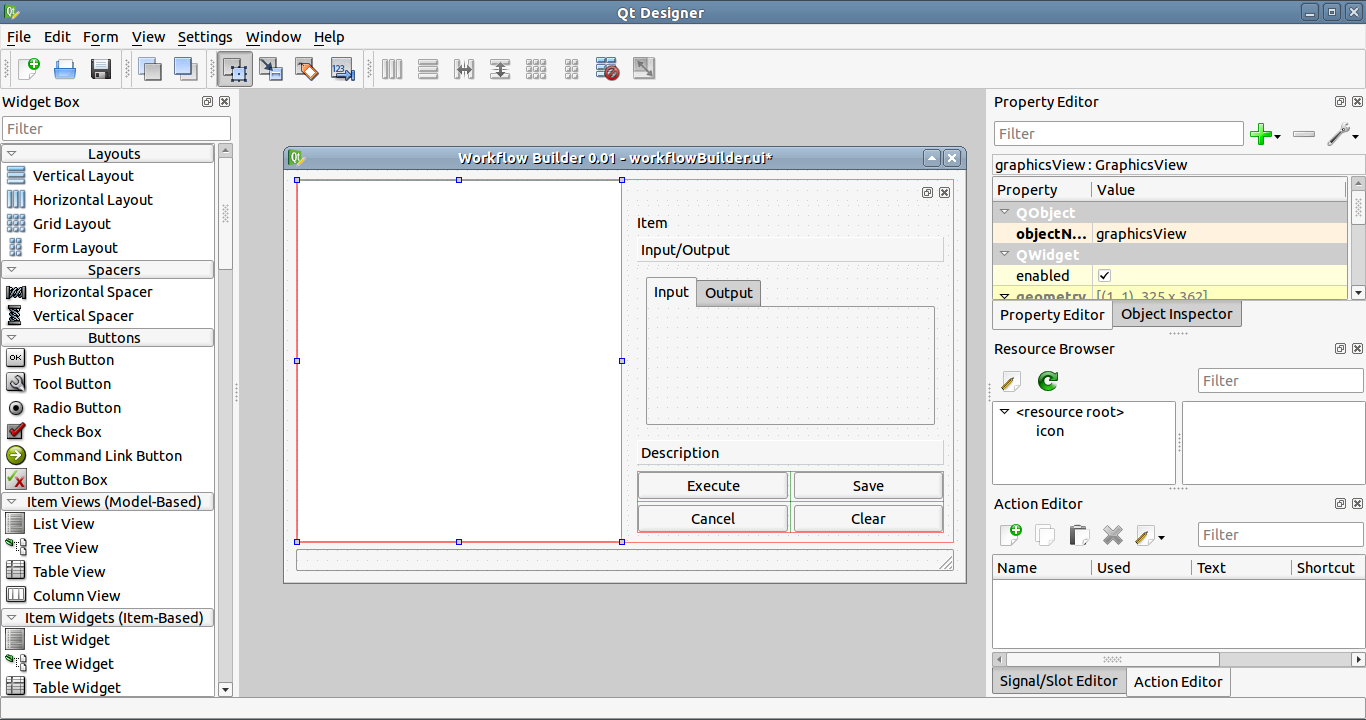
\includegraphics[scale=0.35]{pictures/qt/qt_designer}
	\caption{Qt Designer - nástroj pro tvorbu grafického rozhraní}
  	\label{qtdesigner}
\end{figure}

Soubor vytvořený v Qt Designer (s příponou \textbf{.ui}) lze jednoduše přeložit programem \textbf{pyuic4} do pythoního kódu, který lze poté dále použít. \\

\begin{lstlisting}[label=pyuic4,caption={pyuic4 - přeložení .ui souboru do pythoního kódu}]
		pyuic4 soubor_vytvoreny_v_Qt_Designer.ui -o soubor_v_Pythonu.py 
\end{lstlisting}

\subsection{Model/View Programming}
\subsection{Graphics View Interface}
\subsection{VisTrails, Orange}

%VisTrails is a scientific workflow management system developed at the Scientific Computing and Imaging Institute at the University of Utah that provides support for data exploration and visualization. It is written in Python and employs Qt via PyQt bindings. The system is open source, released under the GPL v2 license. The pre-compiled versions for Windows, Mac OS X, and Linux come with an installer and several packages, including VTK, matplotlib, and ImageMagick. VisTrails also supports user-defined packages.